\subsection{Digital Topology}
\label{sec:digital-topology}

In two dimensions, a black and white image consists of an array of pixels
where each pixel is either black or white.
This idea can be extended to three dimensions,
instead of square pixels we have cubes called voxels.
For example, in medical imaging it is useful to consider
three dimensional images of the human heart \cite{bovik_handbook_2000}.
Given such an image, one might want to compute
the number of holes in the image to make sure it
matches the number of holes that are suppose to be in
the human heart. In \cite{chen_digital_2010}, Chen and Rong 
use the Gauss-Bonnet theorem to efficently
compute genus and Betti numbers of a three dimensional
digital object in $\R^3$. 


We call these digital images \emph{cubical complexes},
where each cube has side length one.
An \emph{elementary cube} $Q$ is a product
$$Q=I_1\times I_2 \times I_3$$
where each $I_i$ is a unit interval of the form $I=[\ell,\ell+1]$
called a \emph{coordinate}.
We will associate each elementary cube with a lattice point.
Given a cubical complex, we would like 
a computer to to classify the image.
Operations toward image classification include
object counting, border following and computing 
the number of holes \cite{kong_digital_1989}.




In two dimensions, it is not clear what it means
for two pixels to be adjacent. See \figref{paradox}
for an ambiguous example. 
We now introduce different notions of adjacency.
In two dimensions, two points are \emph{eight-adjacent}
if they are distinct and each coordinate of one differs from
the other by at most one.
Two points are \emph{four-adjacent} if
they are eight-adjacent and differ in at most one of their coordinates.

In three dimensions, two points
are \emph{26-adjacent} if they are distinct and each coordinate 
entry differs by at most one.
The points are \emph{18-adjacent} if they are 26-adjacent
and different in  a most two of their coordinates.
The points are \emph{6-adjacent} if they are 18-adjacent and differ 
in at most one of their coordinates.

If a set of points $S$ lattice points cannot be
partitioned into two subsets that are not
$n$-adjacent is \EMPH{$n$-connected}.

Consider four vertices adjacent to a single vertex $v$.
If four-adjacency is used the four black points are disconnected,
but separate $v$ from the exterior, if eight-adjacency is used
the back points form a Jordan curve that does not separate
an interior. To resolve this matter, we use eight-adjacency
for the white vertices and four-adjacency for the black.
We make a similar choice in three-dimensions.

\begin{figure}[htb]
        \centering
        \begin{subfigure}[b]{0.35\textwidth}
        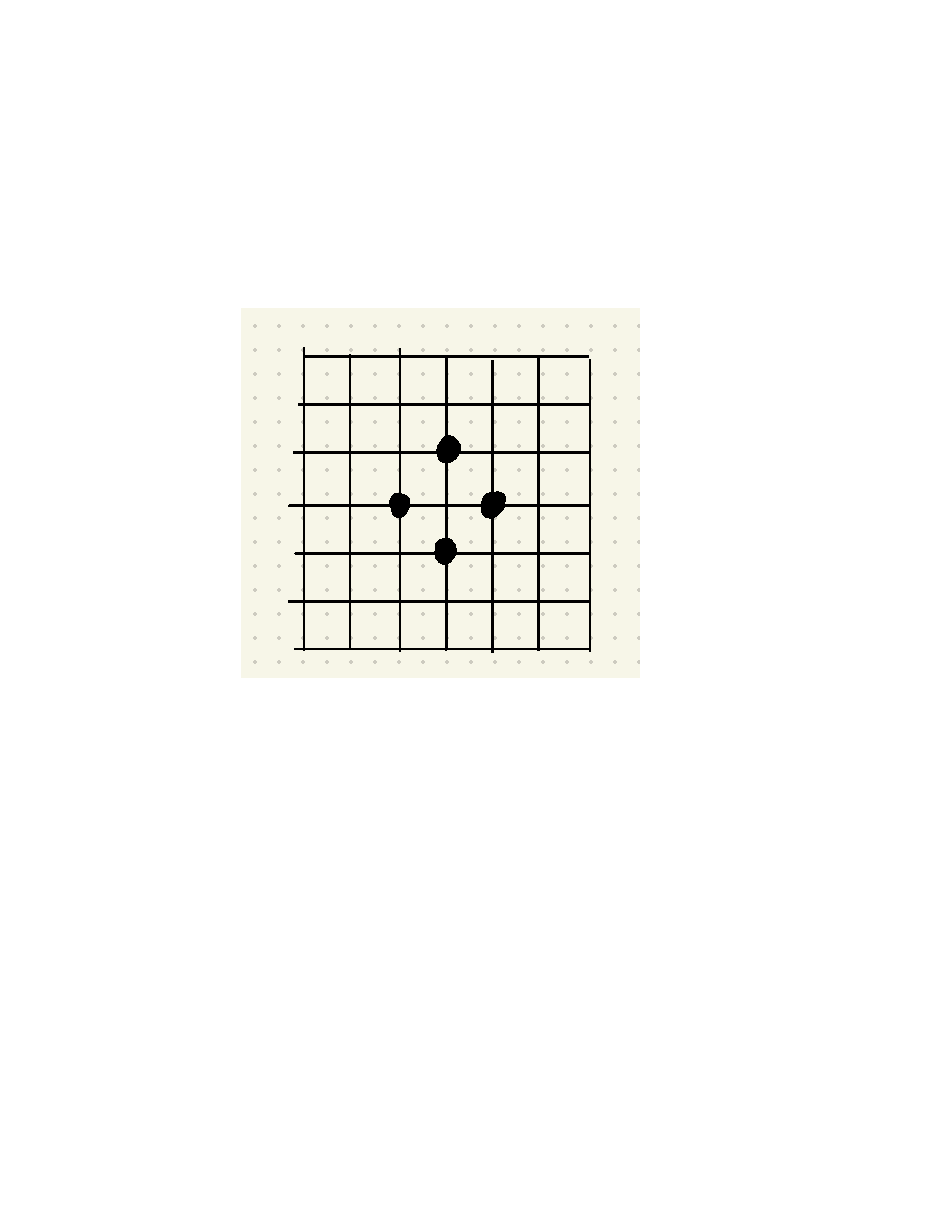
\includegraphics[width=\textwidth]{digital/paradox}
        \caption{}
          \label{fig:paradox}
        \end{subfigure}
          \hspace{.0cm}
         \begin{subfigure}[b]{0.40\textwidth}
        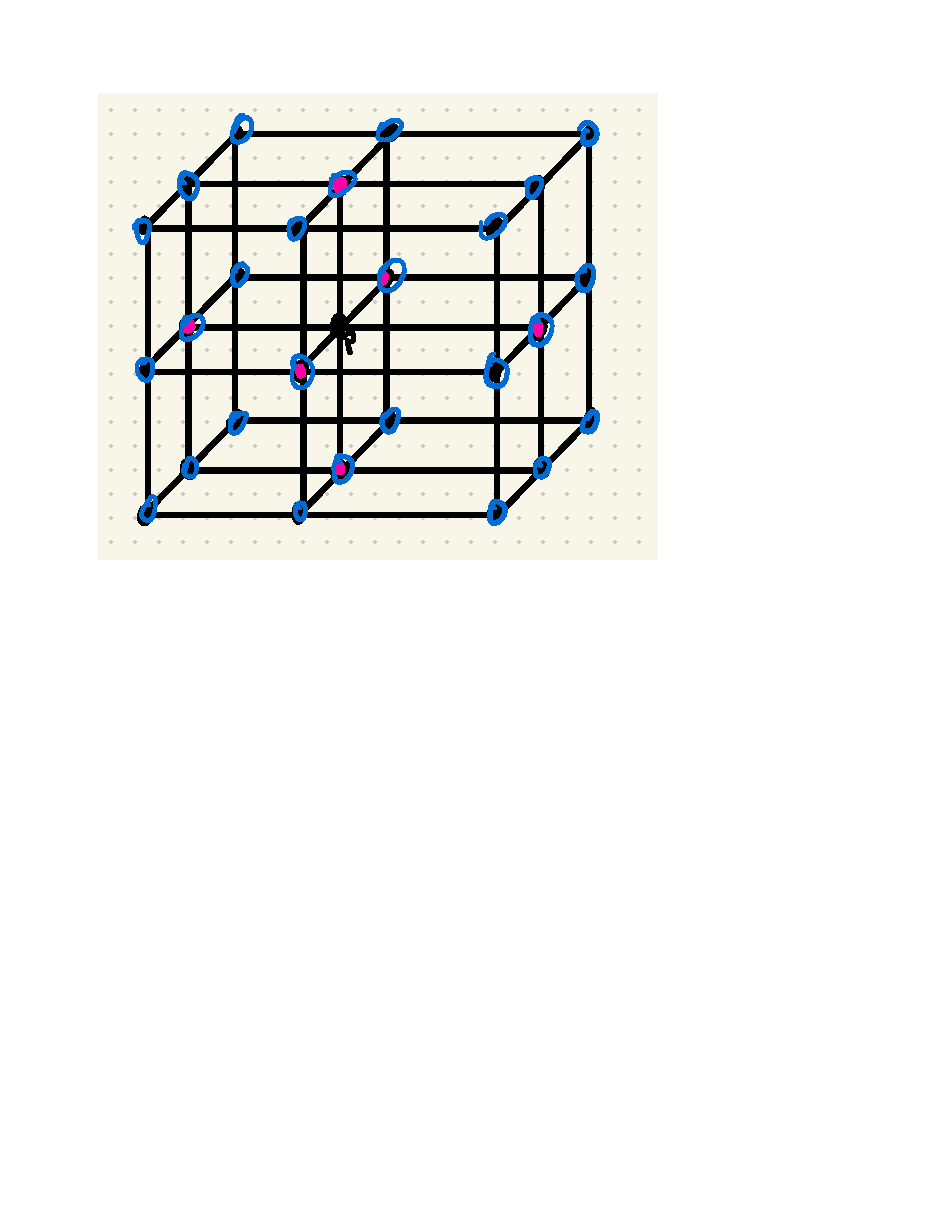
\includegraphics[width=\textwidth]{digital/6-26}
        \caption{}
        \label{fig:6-26}
        \end{subfigure}\\
		\caption{(a) Are the black points a closed curve? (b) In three-dimensions,
		the six neighbors of the vertex $p$ are in pink and the 26 neighbors are in
		blue. 
		\label{fig:adjacency}}
\end{figure}

A \EMPH{digital picture} is a quadruple $(V,m,n,B)$ where
$V=\R^2$ and $(m,n)=(4,8)$ or $V=\R^3$ and $(m,n)=(6,26)$
and $B$ is a subset of $V$. Elements of $B$ are black vertices
and elements not in $V$ are white.


One may ask, why don't we triangulate the cubical complex and
count vertices, edges, and faces to determine the genus.
One reason against doing this is that 
decomposing a cubical complex into a simplicial complex
results in 24 times as many highest dimensional cells \cite{Kaczynski2003}.


We consider cubical spaces in $\R^3$ with $(6,26)$-connectivity,
where two points are adjacent if their Euclidean distance is one.
If $M$ is a closed, orientable digital surface, there are
six types of digital surface points, these are shown in \figref{surface-points}.

\begin{figure}[htb]
        \centering
        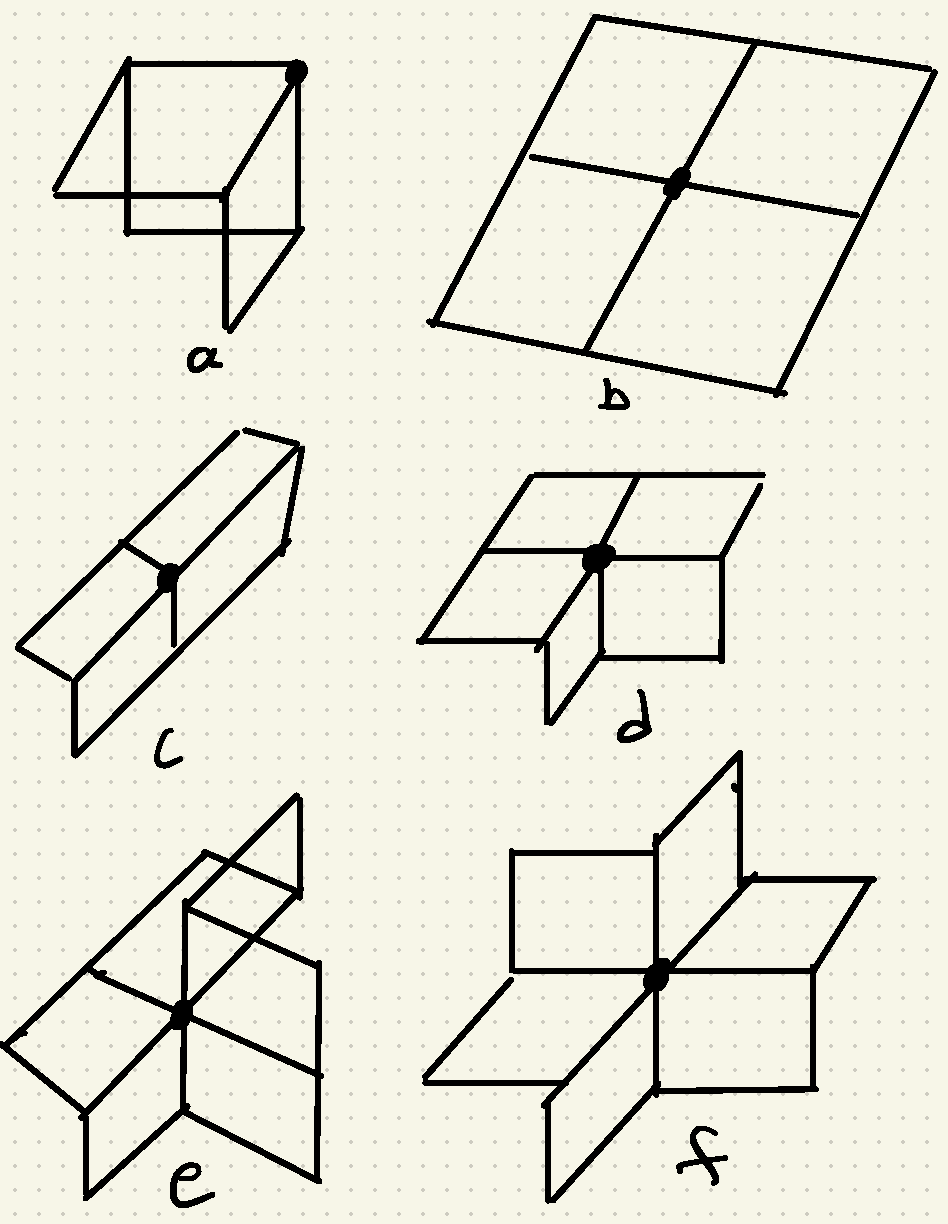
\includegraphics[width=.45\textwidth]{digital/surface-points}
		\caption{
		\label{fig:surface-points}}
\end{figure}

Let $M_i$ denote the set of digital points with $i$ neighbors and $K_i$
the curvature.
Then, by \eqnref{defect}, we have
\begin{enumerate}[(a)]
\item $K_3=\pi/2,$
\item $K_4=0,$
\item $K_5=-\pi/2,$
\item $K_6=-\pi.$
\end{enumerate}

For a closed two-manifold the is the boundary of a three-dimensional
digital image, the Gauss-Bonnet theorem implies
$$\sum_{i=3}^6K_i |M_i|=2(2-2g).$$
A linear time algorithm to compute the genus is the following.
Iterate through all points in $M$ and count the neighbors at each point
and keep track of $M_i$. Then use the above equation to  calculate the genus
using 
$$g=1+(|M_5|+2|M_6|-|M_3|)/8.$$